%%%%% Document Setup %%%%%%%%

\documentclass[12pt, twocolumn]{revtex4}    % Font size (12pt) and column number (one or two).

\usepackage[a4paper, left=2.5cm, right=2.5cm, top=2.5cm, bottom=2.5cm]{geometry}  % Defines paper size and margin length

\renewcommand{\baselinestretch}{1}     % Defines the line spacing

\usepackage{subcaption}

\usepackage[font=small, labelfont=bf]{caption}                      % Defines caption font size and caption title bolded
\captionsetup[figure]{justification=justified, singlelinecheck=off, font=footnotesize} 
\captionsetup{compatibility=false}

\usepackage{graphics,graphicx,epsfig,ulem}	% Makes sure all graphics works
\usepackage{amsmath} 						% Adds mathematical features for equations

\usepackage{etoolbox}                       % Customise date to preferred format
\makeatletter
\patchcmd{\frontmatter@RRAP@format}{(}{}{}{}
\patchcmd{\frontmatter@RRAP@format}{)}{}{}{}
\renewcommand\Dated@name{}
\makeatother

\usepackage{fancyhdr}

\pagestyle{fancy}                           % Insert header
\renewcommand{\headrulewidth}{0pt}
\lhead{\small Jacky Cao}                        
\rhead{\small The relation between stars and gas in distant galaxies}                

\def\thesection{\arabic{section}}
\def\thesubsection{\alph{subsection}}

\def\bibsection{\section*{References}}        % Position reference section correctly


%%%%% Document %%%%%
\begin{document}                     


\title{The relation between stars and gas in distant galaxies} 
\date{Submitted: \today{}}
\author{Jacky Cao}
\affiliation{\normalfont Level 4 Project, MPhys Theoretical Physics\\ Supervisor: Dr.~Mark Swinbank\\ Department of Physics, Durham University}

\begin{abstract}              
 
 Observing any galaxy in the universe will yield the fact that it contains stars and also gas. The dynamics of both can be explored by observing galaxies and collecting spectroscopic data. 
 
Abstract abstract abstract abstract abstract abstract abstract abstract abstract abstract abstract abstract abstract abstract abstract abstract abstract abstract abstract abstract abstract abstract abstract abstract abstract abstract abstract abstract abstract abstract abstract abstract abstract abstract abstract abstract abstract abstract abstract abstract abstract abstract abstract abstract abstract abstract abstract abstract abstract abstract abstract abstract abstract abstract 

\end{abstract}


\maketitle
%\thispagestyle{plain} % produces page number for front page

\tableofcontents
%\let\toc@pre\relax
%\let\toc@post\relax

\newpage

\section{Introduction} 

Amongst the different types of cosmic structure within our universe, galaxies can be seen as the island powerhouses of industry and activity. Containing countless stars, gas, dust, and dark matter \cite{carroll_astro}, it would be difficult not to express the statement that the motions of these objects must be linked in some galactic relationship. 

By utilising the most powerful tool in astronomy, observation, galaxies, their structure and the motions of the objects within them can be studied to a great depth. As an example, if we took optical measurements of the stellar population, we could use that information to estimate the potential age of the galaxy. We know that redder stars are older and bluer stars represent a more young set of objects \cite{carroll_astro}. Or if we wanted to know about the material composition or even the distance to a certain galaxy, we could split the collected light in a spectrograph to produce a spectrum. Values of redshift and the content of a galaxy can be obtained by looking at the absorption and emission lines within a galactic spectrum \cite{carroll_astro}.

Gathering and processing this optical and spectroscopic information allows us to build a broad picture of the internal workings of a galaxy. Then with further analysis we can begin to comprehend the intricate relationships contained within these individual islands. 

To begin with we must consider a general picture of galaxies, after which we will be able to appreciate and explore more complex ideas.

\subsection{Galactic classification}

As we stated previously, a galaxy can be quite broadly defined as a collection of gas, dust, stars and dark matter. But if we were to observe a large enough sample of them then we would begin to see that some of them could potentially be grouped together. 

This categorisation is called the \textit{Hubble Sequence} or the \textit{Hubble Tuning Fork}. With a horizontal handle and two prongs, the sequence itself does not show the evolution of the galaxies, rather it provides a way to view the possible different types of galaxies on one graph. [REF and show an example of the sequence - find some data and plot it? or images of galaxies?] 

We introduced the concept that through optical measurements of the stars 

What do I want to say with this? I want to introduce galaxies, the different types of galaxies, how they form, how they can be confused with other types of structure. 

\subsection{Data} 

-

\subsubsection{HUDF and MUSE}

To obtain spectroscopic information on the Hubble UDF objects, the Multi-Unit Spectroscopic Explorer or MUSE was employed. This instrument is 

what is MUSE, where it is on the VLT, problems, limitations of MUSE - why it is useful...etc

\onecolumngrid

\begin{figure}
  \begin{subfigure}[b]{0.4\textwidth}
    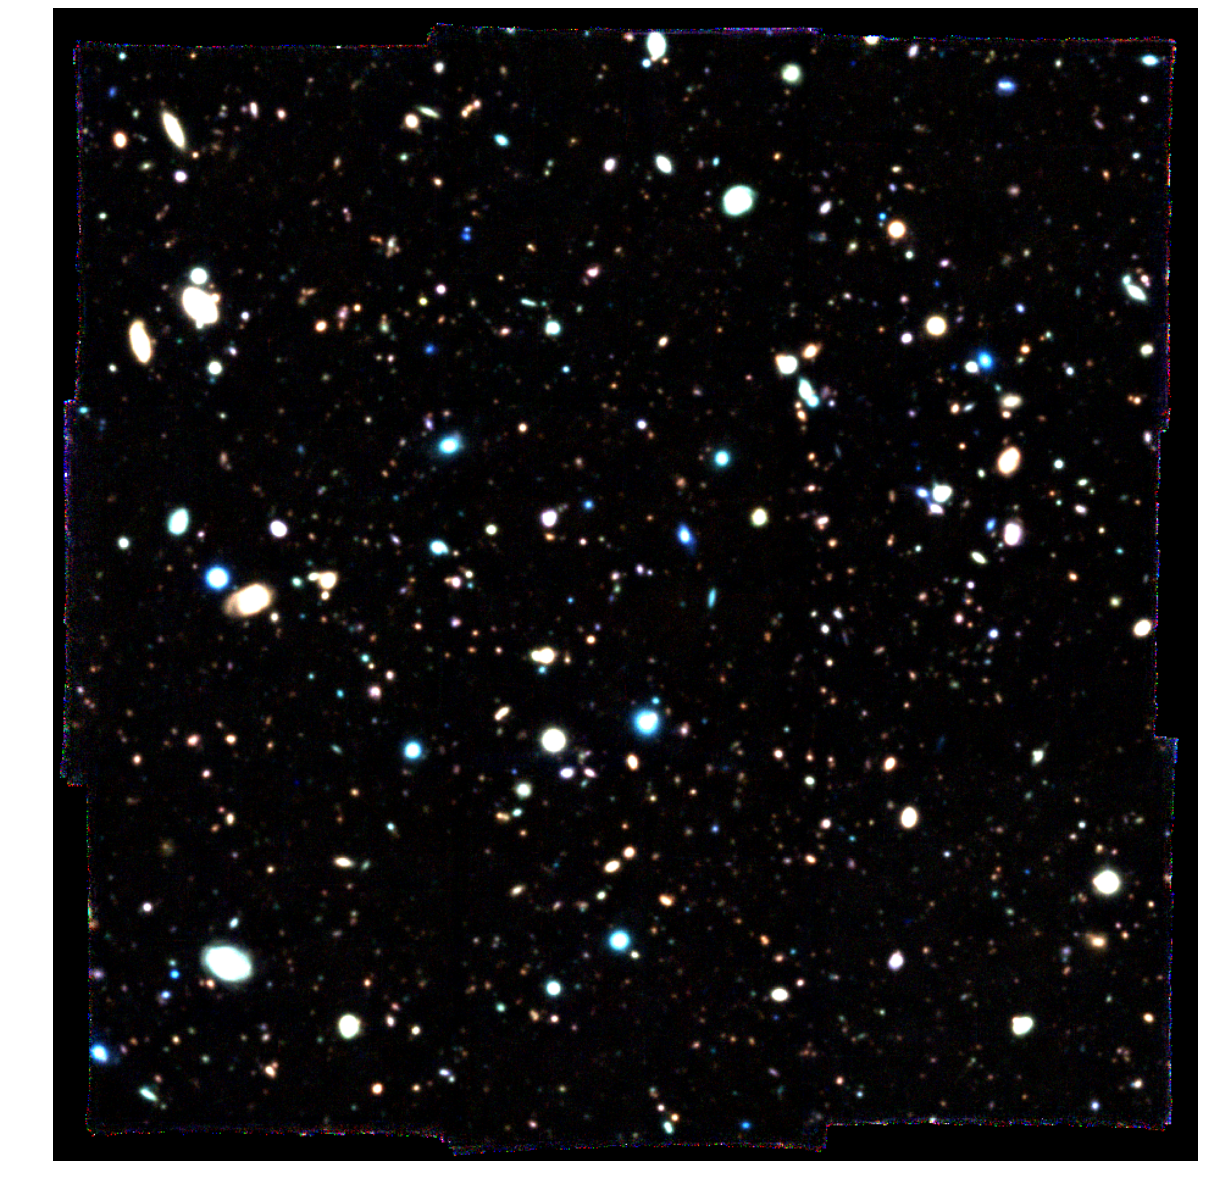
\includegraphics[width=\textwidth]{diagrams/muse_colour_image}
    \caption{MUSE HUDF}
    \label{fig:muse_colour_image}
  \end{subfigure}
  %
  \begin{subfigure}[b]{0.4\textwidth}
    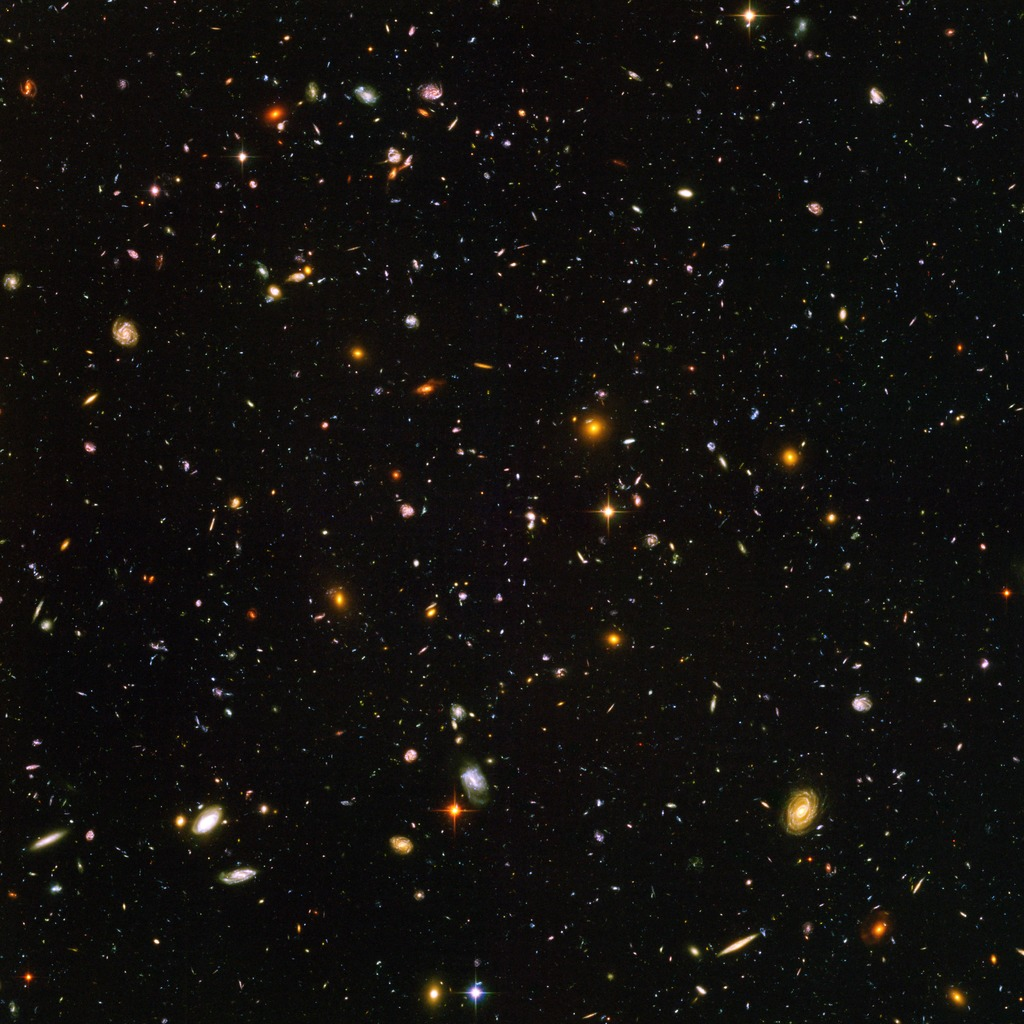
\includegraphics[width=\textwidth]{diagrams/hubble_ultra_deep_field}
    \caption{HST HUDF}
    \label{fig:hubble_ultra_deep_field}
  \end{subfigure}
  \caption[]{(a) A colour image created from the MUSE spectroscopic data of the HUDF. The wavelength range was split into three equal regions and then collapsed to create three bands (R, G, B). A final colour image was produced by combining these separate frames together. (b) The optical HUDF as captured by the Advanced Camera for Surveys instrument on the Hubble Space Telescope \cite{hudf_image}. }
\end{figure}

\twocolumngrid

\section{Analysis} 

\subsection{Cube extraction}

\subsection{pPXF} 

-

\section{Discussion} 

-

\section{Conclusions}
 
In conclusion, through extensive data and statistical analysis it can be said that the dynamics of stars and gas in galaxies are ... (?) 

\begin{acknowledgments}
The author would like to thank Dr.~M.~Swinbank and Dr.~A.~Tiley for their continual help and support throughout the project period, without which, the project would have been experimentally grounded.
\end{acknowledgments}

\bibliographystyle{unsrt}
\bibliography{stars_gas_dynamics}

\end{document}